\documentclass[a4paper]{ltxdoc}
\usepackage{lmodern}			% Usa a fonte Latin Modern			
\usepackage[T1]{fontenc}		% seleção de códigos de fonte.
\usepackage[utf8]{inputenc}		% determina a codificação utiizada (conversão automática dos acentos)
\usepackage{hyperref}  			% controla a formação do índice
\usepackage{parskip}			% espaçamento entre os parágrafos
\usepackage{microtype} 			% para melhorias de justificação
\usepackage{morefloats}			% permite mais floats
\usepackage[absolute]{textpos}
\usepackage{tabularx}
\usepackage[table]{xcolor}
\usepackage{graphicx}
\usepackage{multirow}

% Babel e ajustes
\usepackage[english,brazil]{babel}		% idiomas
\addto\captionsbrazil{
    %% ajusta nomes padroes do babel
    \renewcommand{\bibname}{Refer\^encias}
    \renewcommand{\indexname}{\'Indice}
    \renewcommand{\listfigurename}{Lista de ilustra\c{c}\~{o}es}
    \renewcommand{\listtablename}{Lista de tabelas}
    %% ajusta nomes usados com a macro \autoref
    \renewcommand{\pageautorefname}{p\'agina}
    \renewcommand{\sectionautorefname}{se{\c c}\~ao}
    \renewcommand{\subsectionautorefname}{subse{\c c}\~ao}
    \renewcommand{\paragraphautorefname}{par\'agrafo}
    \renewcommand{\subsubsectionautorefname}{subse{\c c}\~ao}
    \renewcommand{\paragraphautorefname}{subse{\c c}\~ao}
}  

\usepackage{color}
\definecolor{thered}{rgb}{0.65,0.04,0.07}
\definecolor{thegreen}{rgb}{0.06,0.44,0.08}
\definecolor{thegrey}{gray}{0.5}
\definecolor{theshade}{rgb}{1,1,0.97}
\definecolor{theframe}{gray}{0.6}
\definecolor{blue}{RGB}{41,5,195}
% \newcommand{\orientador}{Prof. Dr. Calebe de Paula Bianchini}
\newcommand{\orientador}{Prof. Dr. Pedro Paulo Balbi de Oliveira}
\newcommand\tab[1][1cm]{\hspace*{#1}}
\IfFileExists{listings.sty}{
  \usepackage{listings}
\lstset{%
	language=[LaTeX]TeX,
	columns=flexible,
	basicstyle=\ttfamily\small,
	backgroundcolor=\color{theshade},
	frame=single,
	tabsize=2,
	rulecolor=\color{theframe},
	title=\lstname,
	escapeinside={\%*}{*)},
	breaklines=true,
	commentstyle=\color{thegrey},
	keywords=[0]{\fichacatalografica,\errata,\folhadeaprovacao,\dedicatoria,\agradecimentos,\epigrafe,\resumo,\siglas,\simbolos,\citacao,\alineas,\subalineas,\incisos},
	keywordstyle=[0]\color{thered},
	keywords=[1]{},
	keywordstyle=[1]\color{thegreen},
	breakatwhitespace=true,
	alsoother={0123456789_},
	inputencoding=utf8,
	extendedchars=true,
	literate={á}{{\'a}}1 {ã}{{\~a}}1 {é}{{\'e}}1 {è}{{\`{e}}}1 {ê}{{\^{e}}}1 {ë}{{\¨{e}}}1 {É}{{\'{E}}}1 {Ê}{{\^{E}}}1 {û}{{\^{u}}}1 {ú}{{\'{u}}}1 {â}{{\^{a}}}1 {à}{{\`{a}}}1 {á}{{\'{a}}}1 {ã}{{\~{a}}}1 {Á}{{\'{A}}}1 {Â}{{\^{A}}}1 {Ã}{{\~{A}}}1 {ç}{{\c{c}}}1 {Ç}{{\c{C}}}1 {õ}{{\~{o}}}1 {ó}{{\'{o}}}1 {ô}{{\^{o}}}1 {Õ}{{\~{O}}}1 {Ó}{{\'{O}}}1 {Ô}{{\^{O}}}1 {î}{{\^{i}}}1 {Î}{{\^{I}}}1 {í}{{\'{i}}}1 {Í}{{\~{Í}}}1,
}
\let\verbatim\relax
 	\lstnewenvironment{verbatim}[1][]{\lstset{##1}}{}
}

\usepackage[alf]{abntex2cite}	% citacoes


% COMANDOS PROPRIOS
% \newcommand{\abnTeX}{}
% \newcommand{\abnTeXForum}{}
\newcommand{\abnTeXSite}{}

\title{\protect\parbox{\textwidth}{\protect\centering \textbf{Conservabilidade de estados de autômatos celulares elementares com atualizações assíncronas por prioridade da vizinhança}}}

\author{Marcelo Vironda Rozanti\\\abnTeXSite Felipe Stefanelli de Aguiar Silva\\\abnTeXSite} 

\date{\today}

\hypersetup{
  pdftitle={Conservabilidade de estados de autômatos celulares elementares com atualizações assíncronas por prioridade da vizinhança},
  pdfauthor={Marcelo Vironda Rozanti}{Felipe Stefanelli de Aguiar Silva},
  pdfkeywords={Asynchronous priority-based updating Elementary Cellular Automata, New Kind of Science, Discrete dynamical systems, Number-conserving}, 
  pdfproducer={Marcelo Vironda Rozanti},
  pdfcreator={vim+LaTeX+abnTeX2},
  colorlinks=true,
  linkcolor=black,
  citecolor=black,
  urlcolor=blue
}

% \EnableCrossrefs
\CodelineIndex
% \RecordChanges
\hyphenpenalty=1000

\begin{document}

\thispagestyle{empty}
\huge{\centerline{UNIVERSIDADE PRESBITERIANA MACKENZIE}}

\bigskip
\bigskip

\centerline{\large{FACULDADE DE COMPUTAÇÃO E INFORMÁTICA}}

\makeatletter
\vfill
\large{\centering{\@author}}

\vspace*{\fill}

\large{Conservabilidade de estados de autômatos celulares elementares com}
\large{\centerline{atualizações assíncronas por prioridade da vizinhança}}

\vspace*{\fill}
\large{\centerline{SÃO PAULO}}
\large{\centerline{2019}}

\pagebreak

\large{\centering{\@author}}
\vfill
\large{\centerline{\@title}}
\vfill
\vspace*{\fill}

Orientador: \orientador
\\
\\
\\


\large{\centerline{SÃO PAULO}}
\large{\centerline{2019}}

\begin{textblock}{6}(9,9)
% Projeto do Trabalho de Conclusão de Curso apresentado à Faculdade de Computação e Informática da Universidade Presbiteriana, desenvolvida como requisito parcial para aprovação na disciplina de Metodologia da Pesquisa em Computação, ministrada pelo professor Dr. Everton Knihs, do curso de Ciência da Computação.
\end{textblock}

\maketitle

\begin{abstract}
Autômatos Celulares são sistemas computacionais discretos e abstratos que se têm provado úteis como modelos genéricos de complexidade e representação de diversas dinâmicas em uma varidade de áreas científicas. Estes sistemas podem ser especificados puramente em termos matemáticos e até implementados em estruturas físicas. Muitos deles podem computar funções e resolver problemas algorítmicos. O presente projeto explora um conjunto fundamental deles, chamados Automatos Celulares Elementares com um tipo específico de atualização assíncrona baseada em prioridade da vizinhança com a esperança de encontrar modelos conservativos que podem ser usados em uma variedade de aplicações práticas. 
% O código correspondende a este trabalho pode ser acessado no repositório \url{https://github.com/mvrozanti/TCC}.
\end{abstract}
Palavras-chave: Autômatos celulares elementares com atualização assíncrona por prioridade, New Kind of Science, Sistemas dinâmicos discretos, Conservabilidade

\vfill

\selectlanguage{english}
\begin{abstract}
Cellular Automata are discrete, abstract computational systems that have proved useful as general models of complexity and representations of dynamics on a variety of scientific fields. These systems can be specified in purely mathematical terms and be implemented in physical structures. Many of them can compute functions and solve algorithmic problems. The present project attempts to explore a fundamental subset of them, called Elementary Cellular Automata with a specific kind of neighbourhood-priority-based asynchronous updating in the search of number-conserving models, which can be used for a variety of practical applications. 
%The implementation developed is hosted at \url{https://github.com/mvrozanti/TCC}.
\end{abstract}
Keywords: \@pdfkeywords

\break

\selectlanguage{brazil}
\renewcommand{\contentsname}{\centerline{\Large Sumário}}

\tableofcontents

\listoftables

\listoffigures

\break

\section{INTRODUÇÃO}

% \tab Este projeto teve como objetivo explorar propriedades conservativas em autômatos celulares (ACs) elementares com atualização assíncrona baseada em prioridade da vizinhança. 

\tab Autômatos Celulares (ACs) são uma categoria de sistemas discretos. Pela sua própria simplicidade, esses sistemas têm ocupado uma posição privilegiada no estudo de complexidade nos mais diversos campos da ciência, de biologia teórica a economia entre muitos outros. O desenvolvimento de ACs é tipicamente atribuído a John von Neumann através de suas tentativas de desenvolver um modelo abstrato de autoreprodução biológica. Ao fim de 1950, foi notado que ACs poderiam ser vistos como computadores paralelos \cite[p. 876]{wolfram2002new}. Apesar de falta de investigação científica até 1970, um exemplo de AC se tornou muito famoso por seu comportamento complexo e regras simplesmente descritas inventadas por John Conway, \textit{The Game of Life}, que se popularizou após sua aparição na revista \textit{Scientific American}. 

\tab Desde então, múltiplos estudos compreensivos foram realizados por cientistas ao redor do mundo, destacando os trabalhos feitos por Stephen Wolfram na década de 1980, culminando na publicação do livro A New Kind of Science em que Wolfram apresenta uma coleção de resultados a respeito de ACs, com uma série de descobertas revolucionárias. 
\tab 

% \tab ``Um AC é caracterizado por uma regra de transição de estados, que determina qual será o próximo estado do reticulado do AC, a partir do seu estado atual.'' \cite{oliveira2000unidimensionais}. 

<+> No item \ref{contex}, apresentaremos alguns conceitos básicos referentes à definição dos ACs. 

\subsection{CONTEXTUALIZAÇÃO E RELEVÂNCIA} \label{contex}
\tab No estudo de ACs, há uma inversão do processo de pesquisa tradicional, que consiste de um objetivo a ser atingido através de uma pesquisa. Ele é dado pela identificação de propriedades ou aplicabilidades de um determinado AC, ou de um conjunto deles <forçação?>.

\break

\subsection{OBJETO DE PESQUISA} \label{objetopesq}

\tab O objeto de pesquisa deste trabalho consiste em ACEs 

\subsubsection{PROBLEMA DE PESQUISA} \label{problema}
<+>

\subsection{CONSERVABILIDADE NUMÉRICA} \label{num-conserv}
Segundo \citeonline{boccara2002number}, ``A one-dimensional q-state n-input CA rule f is number-conserving if, for all cyclic configurations of length L \(\geq\) n, it satisfies'':

\[f(x_1,x_2,...,x_{n-1},x_n) + f(x_2,x_3,...,x_n,x_{n+1}) + ... \]
\tab \[ + \;   f(x_L,x_1,...,x_{n-2},x_{n-1} = x_1 + x_2 + ... + x_L\]
% \tab Muitos algoritmos de classificação, no que é pertinente ao campo de Machine Learning, se utilizam de medidas de similaridade tanto para o ``treino'' destes classificadores, como para o seu uso em produção. Estes algoritmos, por sua vez, requerem alto custo computacional. Pode-se criar uma solução mais eficiente que as atuais em arquiteturas paralelas de 512-bit? Ainda, como adaptar a solução a arquiteturas com maior largura de registradores? 

\break

% \subsubsection{FÓRMULAS UTILIZADAS} \label{formulas}

% \break

% \tab Estas operações são usadas constante e intensivamente em algoritmos pertinentes ao domínio de Machine Learning como explicitado por \citeonline{wang2012distance} que ressaltam, ainda, o problema da Maldição da Dimensionalidade, também conhecido pelo anglicismo \textit{Curse of Dimensionality}, sendo possível depreender a importância da eficiência da implementação dos cálculos mencionados.

\subsubsection{HIPÓTESE BÁSICA} 

\tab Dados os esquemas de atualização mencionados na seção \ref{objetopesq}, encontrar quais esquemas apresentaram conservabilidade numérica <<isso nao eh uma hipotese>>.

\subsubsection{VARIÁVEIS} \label{varia}

\begin{itemize}
	\item Largura do reticulado:\\
          \tab A largura do espaço de regras.
	\item Espaço Celular:\\
	\item Regra de transição:\\
	\item Timesteps:\\

\end{itemize}

\subsection{OBJETIVOS DO ESTUDO} 
% \tab O objetivo desse estudo é ganhar maior compreensão sobre as capacidades e limitações encontradas no design eficiente de implementações em arquiteturas paralelas, bem como ampliar o conhecimento sobre compiladores e tradução código-máquina.

\subsubsection{OBJETIVO GERAL}
% \tab Tornar algoritmos-base de cálculo de distância mais eficientes em determinadas arquiteturas.
\subsubsection{OBJETIVOS ESPECÍFICOS}
<+>

% \tab Para alcançar o objetivo geral proposto para a resolução do problema de pesquisa, 
% os seguintes objetivos específicos foram estabelecidos:

% \begin{itemize}
    % \item Identificação das  teorias  envolvidas  no  estudo  de  otimização  os aspectos que privilegiam o processo de desenvolvimento das otimizações. 
    % \item Estudo no âmbito computacional atual dos processos de técnicas e boas práticas de otimização. 
    % \item Identificação dos aspectos que qualificam alta-performance que devem ser observados na criação e desenvolvimento destes algoritmos. 
% \end{itemize}

\subsection{JUSTIFICATIVA}
<+>
% \tab Como já mencionado no item \ref{problema}, os algoritmos de classificação podem usar intensamente o cálculo de distância como instrumento intermediário e têm um impacto direto em sua performance. Qualquer ganho de eficiência nestes algoritmos de cálculo de distância em função da arquitetura pode ter uma influência notável na performance geral  dos classificadores em fase de treinamento ou em fase prática, ou, de produção, como afirmam \citeonline{effective-simd-vectorization} e \citeonline{optimization-pattern-recognition}.

\subsection{DELIMITAÇÃO DO ESTUDO} \label{delimitacao}
<+>
% \tab Deve-se restringir a implementação dos algoritmos evidenciados no item \ref{problema}:

% \begin{itemize}
%     \item Delimitação Organizacional: família Intel® de processadores
%     \item Delimitação por Indicadores de Desempenho: testes com o intuito de verificar a eficiência do código proposto.
% \end{itemize}

% \break

\subsection{ORGANIZAÇÃO DO ESTUDO}

Descrição dos capítulos:

\begin{enumerate}
    \item Introdução
        \subitem Preâmbulo deste trabalho.
    \item Referencial Teórico
        \subitem Sustentação argumentativa sobre o tema proposto.
    \item Metodologia de Pesquisa
        \subitem Sistematização dos instrumentos e processos de estudo empregados no presente trabalho.
    \item Cronograma
        \subitem Planejamento das tarefas necessárias para a conclusão deste trabalho, bem como suas expectativas de início e conclusão.
    % \item Descrição da plataforma-alvo.
    %     \subitem Breve narrativa sobre ambiente e ferramentas utilizadas ao longo do estudo.
    % \item Implementações de cálculo de distância.
        % \subitem Detalhamento da solução final.
\end{enumerate}
 
\section{REFERENCIAL TEÓRICO}
\tab Em relação ao referencial teórico estudado neste TCC, foi de suma importância entender os seguintes tópicos:

\subsection{AUTÔMATOS CELULARES ELEMENTARES} \label{aces}
<+>
% \tab 

\subsubsection{AUTÔMATOS CELULARES}

Um AC pode ser descrito simplesmente por seu \textit{espaço celular} e \textit{regra de transição} segundo \citeonline{oliveira2000unidimensionais}: 

``O \textit{espaço celular} é um reticulado de N células idênticas, cada qual com um padrão idêntico de conexões locais para outras células e com condições de contorno. O conjunto de estados possíveis da célula é denotado por \(\Sigma\) e o número de estados desse conjunto é denotado por \textbf{k}. Cada célula é denotada por um índice \textbf{i} e seu estado a um dado tempo \textbf{t} é denotado por \(n_i^t\), onde \(S_i^t \in \Sigma\). O estado \(S_i^t\) da célula \textbf{i} e os estados das células às quais a célula \textbf{i} está conectada são chamados de vizinhança \(n_i^t\) da célula \textbf{i}.''


% (como é descrito\ref{varia}).

\subsection{AUTÔMATOS CELULARES ELEMENTARES}


\tab Visualização:

\begin{figure}[!htbp]
\centerline{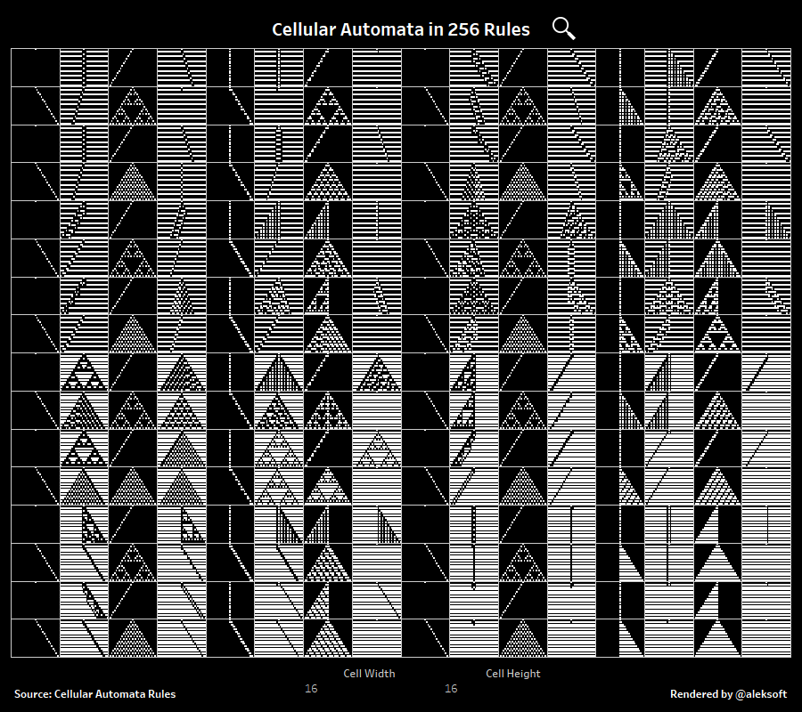
\includegraphics[width=\linewidth/2]{imgs/Picture1.png}}
\caption{Ilustração das 256 regras elementares}
\end{figure}

\subsubsection{REPRESENTAÇÕES}

<+>

Então, para ACs de 1 dimensão, elementares, com vizinhança \texttt{\{-1,0,1\}}, com conjunto de estados \texttt{\{0,1\}}, na ordem lexicográfica \{\textit{\(w_0\)}, ..., \textit{\(w_7\)},\} em \(\{0,1\}^3\), se \(\delta(\textit{w}_i)=s_i,s_0,...s_7\) representa \(\delta\). Analogamente, qualquer inteiro positivo menor que 256 = \(2^8\) define um ACE \cite[cap. 2]{delorme1999introduction}.

\begin{figure}[!htbp]
\centerline{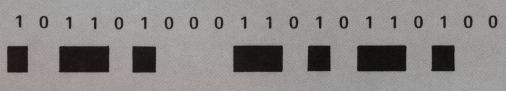
\includegraphics[width=\linewidth/2]{imgs/typical-config.png}}
\caption{Nas renderizações, é convenção representar 1s como células em preto e 0s em branco. \cite{wolfram2002new} }
\end{figure}

\begin{figure}[!htbp]
\centerline{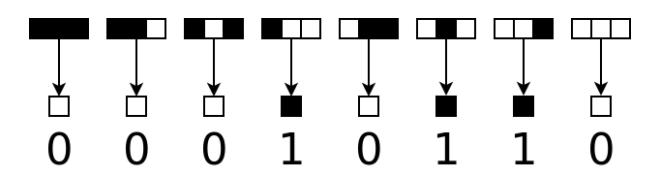
\includegraphics[width=\linewidth/2]{imgs/rule_22.png}}
\caption{Ilustração do mapa de transições para a regra 22 na notação de \citeonline{wolfram1983cellular}}
\end{figure}

\begin{figure}[!htbp]
\centerline{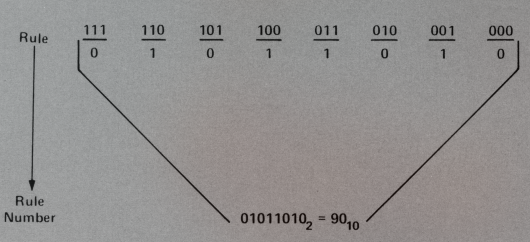
\includegraphics[width=\linewidth/2]{imgs/rule-transitions.png}}
\caption{Ilustração do mapa de transições para a regra 90 na notação de \citeonline{wolfram1983cellular}}
\end{figure}

\subsubsection{TIPOS DE ATUALIZAÇÃO} \label{tiposatt}
<+>

\section{METODOLOGIA DA PESQUISA}
\tab No que tange à Metodologia empregada neste TCC, o trabalho teve início com uma revisão da literatura específica sobre o tema da pesquisa. Esta pesquisa abrange conceitos fundamentais de teoria da computação e o "estado da arte" em termos de análise de conservabilidade.

Este alicerce teórico foi obtido através de autores como: Wolfram; Oliveira;
entre outros, além de pesquisas em periódicos científicos, sites, publicações em empresas, teses e dissertações em universidades e publicações de associações técnicas.  A leitura, análise e comparação da fundamentação teórica tiveram início com ACEs síncronos, modificados em seguida para viabilizar o tipo de atualização mencionado no item \ref{tiposatt}.


\subsection{ETAPAS DA PESQUISA}
\tab Para definir as etapas da pesquisa, foi necessário atender às delimitações de estudo (item \ref{delimitacao}), desenvolvendo uma implementação que atendesse à execução dos ACE com esquemas distintos <+>, como descrito no Cronograma apresentado no item \ref{cron}.

\break

Assim, pode-se dizer que as etapas desenvolvidas neste estudo foram:

\begin{enumerate}
    \item Estudo do estado da arte;
    \item Implementação do simulador para execuções síncronas;
    \item Implementação do renderizador;
    \item Implementação do simulador para execuções assíncronas;
    \item Implementação do verificador de evoluções conservativas;
    \item Análise e testes das implementações;
    \item Análise dos resultados;
    \item Artigo.
\end{enumerate}

\subsubsection{CONCEITOS EMPREGADOS}
<+>

\begin{itemize}
  \item 
\end{itemize}

\subsection{CLASSIFICAÇÃO DA PESQUISA}
\tab O tempo total previsto para a conclusão desta pesquisa é de 1 ano, como mostrado no capítulo \ref{cron}.

\subsubsection{NATUREZA DA PESQUISA}
\tab Esta é uma pesquisa exploratória, dada a natureza desconhecida das propriedades de ACEs com esse tipo de atualização.

\subsubsection{ABORDAGEM} 
\tab Esta pesquisa é baseada em cálculos, medidas objetivas e dados verificáveis.

\subsubsection{FINS} 
\tab Esta pesquisa foi voltada para encontrar caminhos, formas, maneiras e procedimentos para atingir um determinado fim, buscando definir um processo ou uma ferramenta que leve à solução do problema proposto (\ref{problema}).

\subsubsection{PESQUISA PROPOSITIVA} 
% \tab Código-fonte, bem como suas instruções de compilação e documentação interna e externa utilizada para gerar o binário que ultrapasse soluções atuais para cálculo de distância nas arquiteturas alvo.

\subsubsection{MEIOS} 
\tab Quanto aos meios, foram utilizados os recursos mencionados na Bibliografia.

\subsubsection{PESQUISA BIBLIOGRÁFICA}

% \vfill
\break
\section{CRONOGRAMA} \label{cron}

\tab As atividades desta pesquisa se desenvolveram de acordo com o cronograma apresentado a seguir, no prazo de 12 meses:

\begin{table}[h]
    \caption{Cronograma de atividades}
    \centerline{
        \begin{tabular}{|l|l|l|l|l|l|l|l|l|l|l|l|l|}
          \hline
          \multirow{2}{*}{ATIVIDADE}                              & \multicolumn{12}{|c|}{MÊS} \\
          % \hline
                                                                  & 1                             & 2                  & 3                  & 4                  & 5                  & 6                  & 7                  & 8                  & 9                  & 10                 & 11                 & 12 \\
          \hline
          Estudo do estado da arte                                & \cellcolor{yellow}            & \cellcolor{yellow} &                    &                    &                    &                    &                    & \cellcolor{yellow} &                    &                    &                    & \\
          \hline
          Implementação do simulador para execuções síncronas     &                               & \cellcolor{yellow} & \cellcolor{yellow} &                    &                    &                    &                    &                    &                    &                    &                    & \\
          \hline
          Implementação do renderizador                           &                               & \cellcolor{yellow} & \cellcolor{yellow} &                    &                    &                    &                    &                    &                    &                    &                    & \\
          \hline
          Implementação do simulador para execuções assíncronas   &                               &                    &                    & \cellcolor{yellow} & \cellcolor{yellow} &                    &                    &                    &                    &                    &                    & \\
          \hline
          Implementação da verificador de evoluções conservativas &                               &                    &                    & \cellcolor{yellow} & \cellcolor{yellow} &                    &                    &                    &                    &                    &                    & \\
          \hline
          Análise e testes das implementações                     &                               &                    &                    &                    &                    & \cellcolor{yellow} & \cellcolor{yellow} &                    &                    &                    &                    & \\
          \hline
          Análise dos resultados                                  &                               &                    &                    &                    &                    & \cellcolor{yellow} & \cellcolor{yellow} & \cellcolor{yellow} & \cellcolor{yellow} & \cellcolor{yellow} &                    & \\
          \hline
          Artigo                                                  &                               &                    &                    &                    &                    &                    &                    & \cellcolor{yellow} & \cellcolor{yellow} & \cellcolor{yellow} & \cellcolor{yellow} & \cellcolor{yellow}\\
          \hline
    \end{tabular}
  }
\end{table}

% \break

\addcontentsline{toc}{section}{Referências}
\bibliography{cellz} \label{bib}

\end{document}
